\documentclass[a4j]{celb-report}
\usepackage{amsmath,amssymb}
\usepackage{comment}
\usepackage[dvipdfmx]{graphicx}
\usepackage[utf8]{inputenc}
\usepackage{listings,jlisting}
\usepackage{type1cm}
%%%
%%% 計算機工学実験Bレポートテンプレート
%%%  このテンプレートを使う場合,celb-report.clsとjlisting.styが必要です.
%%%  このファイルと同じディレクトリに置いておいてください.
%%%

%%%
%%% まずはここで各種設定
%%%
\period{1} % ← 何回目のレポートか(1~3)
\stunum{S153012} % ← 学生番号
\author{学生 伊藤 太清} % ← 学生氏名
\date{\today} % ← レポート提出日
\lstset{%
	basicstyle={\small\ttfamily},%
	tabsize=8,
	identifierstyle={\small},%
	commentstyle={\small\itshape},%
	keywordstyle={\small\bfseries},%
	ndkeywordstyle={\small},%
	stringstyle={\small\ttfamily},
	frame={tb},
	breaklines=true,
	columns=[1]{fullflexible},%
	numbers=left,%
	xrightmargin=0zw,%
	xleftmargin=3zw,%
	numberstyle={\scriptsize},%
	stepnumber=1,
	numbersep=1zw,%
	lineskip=-0.5ex,%
	keepspaces=true,
	showstringspaces=false
}
\begin{document}

\maketitle

%%%%%%%%%%%%%%%%%%%%%%%%%%%%%%%%%%%%%%%%%%%%%%%%%%%%%%%%%%%%%%%%%%%%%
% レポート作成の手引:
%   レポート提出時は、ここから「レポート作成の手引ここまで」までの行をすべて削除すること!
%%%%%%%%%%%%%%%%%%%%%%%%%%%%%%%%%%%%%%%%%%%%%%%%%%%%%%%%%%%%%%%%%%%%%
\begin{comment}
\setcounter{section}{-1}
\section{レポート作成の手引}

各レポート,対応する回ごとに章(\verb|\section|)に分け,テキストの報告内容にて指示されている課題ごとに節(\verb|\subsection|)を用意して記載する.次章にて第1回分の例を記載しているので,適宜参考にすること.

% ----------------------------------------------------
\subsection{プログラムのソースコード,実行結果等を掲載する場合}

プログラムのソースコードや実行結果等を貼り付ける場合は,\verb|\lstlisting|環境を用いると良い.使い方は,このファイルの\texttt{tex}ソースを参考にすること.基本的には,ソースに記載の内容をコピーし,実行結果を書き換えると良い.
%
% --- 実行結果ここから
\begin{lstlisting}[basicstyle=\ttfamily\footnotesize, frame=single]

※※ ここに実行結果を貼り付ける. ※※
 
\end{lstlisting}
% --- 実行結果ここまで
%

% ----------------------------------------------------
\subsection{課題}

各回で用意されている考察・調査課題については,\verb|\kadai|を用いて,課題文と回答を記載する.第1回分の例を参考にすること.

% ----------------------------------------------------
\subsection{図の貼り付け}

図を貼り付ける場合は,\verb|\figure|環境を用いる.基本的には,このファイルの\texttt{tex}ソース内にある記述をそのまま用いれば良い.\verb|\includegraphcs|で画像ファイルを指定し,\verb|\caption|で図にキャプションを付ける.\verb|\label|は,本文中で図番号を参照するために付けておくラベルである(詳しくは後述).
%
\begin{figure}[htb]
 \centering 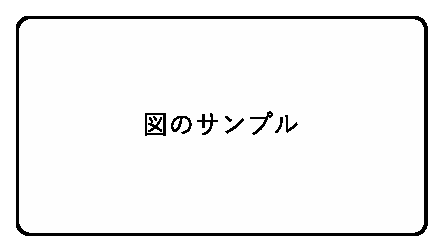
\includegraphics[scale=0.8]{sample-figure.eps}
 \caption{図のサンプル} \label{fig:sample}
\end{figure}
%

本文中で図を引用する場合は,図中で指定した\verb|label|を\verb|\ref|を用いて参照する.例えば上図で\verb|\label{fig:sample}|としている状態で本文中に``図\verb|\ref{fig:sample}|''と記述すると,texコンパイル後のファイルでは当該箇所が``図\ref{fig:sample}''に変換される.``図??''となる場合は,もう1度texコンパイルしてみて,それでも参照がされない場合は,ラベルが一致しているかどうか確認する.

% ----------------------------------------------------
\subsection{(第3レポートのみ)グループ内の役割分担}

第3レポートの対象となる回では,複数人のグループで作業を行うため,各回で誰が何を担当したのかも節(\verb|\subsection|)を用いて記載する.以下は記載例である.\texttt{tex}ソースに記載の通り,\verb|\description|環境を用いると良い.
%
\begin{description}
 \item[s123456 学生 なまえ] ネットワークの配線,環境の構築
 \item[s135791 相方 ひとりめ] プログラムのコーディング,デバッグ
 \item[s246802 相方 ふたりめ] コーディングのサポート
 \item[s369258 相方 さんにんめ] 3人の応援
\end{description}

% ----------------------------------------------------
\subsection{参考文献等}

書籍,インターネット上の情報などを参考にした場合,対象となるすべての回のものをまとめて,\verb|\thebibliography|環境を用いて出展を明記する.書き方は本ファイルの\texttt{tex}ソースを参考にする.
%
\end{comment}
%%%%%%%%%%%%%%%%%%%%%%%%%%%%%%%%%%%%%%%%%%%%%%%%%%%%%%%%%%%%%%%%%%%%%
% レポート作成の手引ここまで
%%%%%%%%%%%%%%%%%%%%%%%%%%%%%%%%%%%%%%%%%%%%%%%%%%%%%%%%%%%%%%%%%%%%%


%%%%%%%%%%%%%%%%%%%%%%%%%%%%%%%%%%%%%%%%%%%%%%%%%%%%%%%%%%%%%%%%%%%%%
% 第1回分(第1レポート内)サンプル
%   第1レポートでは,第1回~第4回分それぞれを 章 (\section) として1つのレポートにまとめること
%%%%%%%%%%%%%%%%%%%%%%%%%%%%%%%%%%%%%%%%%%%%%%%%%%%%%%%%%%%%%%%%%%%%%
%%% ------------------------------------------------------------------
%\newpage % ← 改ページ
\section{第1回 誤り制御符号(1):パリティ符号}

% ----------------------------------------------------
\subsection{実行結果}

%
% --- 実行結果ここから
\begin{lstlisting}[basicstyle=\ttfamily\footnotesize, frame=single]

********
  1ビット垂直パリティ検査を体験するプログラムです。
  7ビットの情報語に1ビットの検査語を加えて伝送します。
  ここでは偶数パリティを使用しています。
********

情報語を10進数で入力してください(0?127  エンターのみで終了): 入力値(10進数) = 12
入力値( 2進数) = 0001100

送信データ 0001100 0  (f6f5f4f3f2f1f0 p0)
受信データ 0001100 0  (f6f5f4f3f2f1f0 p0)
  算出された検査ビット = 0

伝送誤りはありません。

情報語を10進数で入力してください(0?127  エンターのみで終了): 入力値(10進数) = 12
入力値( 2進数) = 0001100

送信データ 0001100 0  (f6f5f4f3f2f1f0 p0)
受信データ 0000111 0  (f6f5f4f3f2f1f0 p0)
  算出された検査ビット = 1

伝送誤りが検出されました。

情報語を10進数で入力してください(0?127  エンターのみで終了): 入力値(10進数) = 12
入力値( 2進数) = 0001100

送信データ 0001100 0  (f6f5f4f3f2f1f0 p0)
受信データ 0001001 0  (f6f5f4f3f2f1f0 p0)
  算出された検査ビット = 0

伝送誤りはありません。

\end{lstlisting}
% --- 実行結果ここまで
%

\subsection{実行結果に対する考察}
%前節の実行結果より,~であることがわかる.また,~であるものと考えられる.
一回目の実行結果では、送信データと受信データは一致し、送受信が成功したことがわかる。\\
二回目の実行結果では、送信データと受信データは一致せず、送受信が失敗していたが、受信データには奇数個の1が含まれているため、伝送誤りを検出することができている。\\
三回目の実行結果では、伝送誤りが発生したが、1が偶数個含まれているので、受信側が伝送誤りを検出していない。これらの結果より、1ビット垂直パリティでは、伝送誤りを検出することはできるが、検出できない時もあることがわかった。


% ----------------------------------------------------
\subsection{課題} 

\kadai{今回の実験で作成したパリティ符号は,偶数パリティと奇数パリティのいずれであるかを答えよ.}

符号内の1の個数を偶数子に保つものであるため,偶数パリティである.

\kadai{1ビット水平パリティ符号について調査せよ.}

%1ビット水平パリティ符号とは,~~ものである.~~.
1ビット垂直パリティ符号はひとつの符号語の中の1の個数を数え、それに応じて0か1かが決定されるが、1ビット水平パリティ符号の場合はいくつかの符号語の中の同じnビット目の中に1がいくつあるか数え、それに応じて、nビット目が0か1かを決定した符号語を追加する方法である。

\kadai{1ビット水平パリティ符号と1ビット垂直パリティ符号を組み合わせることにより,1ビットの誤りを訂正できることを示せ.}

いくつかの符号語を送信し、1ビットの誤りが発生した時、各符号語の垂直パリティビットのうち、伝送誤りが検出されるものが必ず一つあり、水平パリティビットが集まった符号語の中にも伝送誤りが検出されるものが必ず一つある。垂直パリティビットの伝送誤りによりどの符号語で誤りが発生したのかがわかり、水平パリティビットの伝送誤りにより誤りが発生した符号語の中の何ビット目に誤りがあるのかがわかる。よって、1ビット水平パリティ符号と1ビット垂直パリティ符号を組み合わせることで1ビットの誤りを訂正することができる。
%
%%%%%%%%%%%%%%%%%%%%%%%%%%%%%%%%%%%%%%%%%%%%%%%%%%%%%%%%%%%%%%%%%%%%%
% 第1回分サンプルここまで
%%%%%%%%%%%%%%%%%%%%%%%%%%%%%%%%%%%%%%%%%%%%%%%%%%%%%%%%%%%%%%%%%%%%%

%%% ------------------------------------------------------------------
\newpage
\section{第2回 誤り制御符号(2):CRC符号の実験}
\subsection{実行結果}
\begin{lstlisting}[basicstyle=\ttfamily\footnotesize, frame=single]

********
  CRC符号の符号化と復号化を体験するプログラムです。
  4ビットの情報語に3ビットの検査語を加えて伝送します。
********

情報語を10進数で入力してください(0?15  エンターのみで終了): 入力値(10進数) = 10
送信データ 1010 011  (f3f2f1f0 r2r1r0)
受信データ 1011 011  (f3f2f1f0 r2r1r0)
    シンドローム 0 1 1  (s2 s1 s0) 
    誤り発生位置 = 3  (f0)
訂正データ 1010 011  (f3f2f1f0 r2r1r0)

情報語を10進数で入力してください(0?15  エンターのみで終了): 入力値(10進数) = 10
送信データ 1010 011  (f3f2f1f0 r2r1r0)
受信データ 1010 011  (f3f2f1f0 r2r1r0)
    シンドローム 0 0 0  (s2 s1 s0) 
    誤りなし
訂正データ 1010 011  (f3f2f1f0 r2r1r0)

\end{lstlisting}
\subsection{実行結果に対する考察}
CRC符号では1ビットの符号誤りが発生した場合でも誤りが発生したビットを特定することができるので、今回の実験結果に送信データと受信データが異なるパターンは現れなかった。しかし、今回のプログラムのような誤り発生位置の特定は誤りが発生した符号がひとつ以下であるという仮定に基づいているので、2ビット以上の誤りが発生した場合は、符号語を訂正することができなくなることが推測される。
\subsection{課題}
生成多項式$ G \left( x \right) = x ^3 + x + 1 $を用いて4ビットの情報語$ \left( 0101 \right) _2 $から7ビットの符号語を生成するとき、符号語が$ G \left( x \right) $で割り切れることを示せ。また、符号語のどこか1ビットを変更した語を作成し、これが$ G \left( x \right) $で割り切れないことを示せ。\\
\\
$ G \left( x \right) $を2進数で表したものを$ g = \left( 1011 \right) _2 $、4ビットの情報語を$ i = \left( 0101 \right) _2 $とする。$ G \left( x \right) $は3次式なので、$ i $を3回左シフトさせたものを$ g $で割ると、
\begin{equation}
	\left( 0101000 \right) _2 \div \left( 1011 \right) _2 = \left( 100 \right) _2 \cdots \left( 100 \right) _2 \nonumber
\end{equation}
よって符号語$ c $は、
\begin{equation}
	c = \left( 0101000 \right) _2 + \left( 100 \right) _2 = \left( 0101100 \right) _2 \nonumber
\end{equation}
となる。この符号語$ c $を$ g $で割ると、
\begin{equation}
	c \div g = \left( 0101100 \right) _2 \div \left( 1011 \right) _2 = \left( 100 \right) _2 \cdots 0 \nonumber
\end{equation}
となり、$ c $は$ g $で割り切れる。\\
また、$ c $のどこか1ビットを変更した語を$ g $で割ると、
\begin{eqnarray}
	\left( 1101100 \right) _2 \div \left( 1011 \right) _2 & = & \left( 1111 \right) _2 \cdots \left( 101 \right) _2 \nonumber \\
	\left( 0001100 \right) _2 \div \left( 1011 \right) _2 & = & \left( 1000 \right) _2 \cdots \left( 111 \right) _2 \nonumber \\
	\left( 0111100 \right) _2 \div \left( 1011 \right) _2 & = & \left( 110 \right) _2 \cdots \left( 110 \right) _2 \nonumber \\
	\left( 0100100 \right) _2 \div \left( 1011 \right) _2 & = & \left( 101 \right) _2 \cdots \left( 11 \right) _2 \nonumber \\
	\left( 0101000 \right) _2 \div \left( 1011 \right) _2 & = & \left( 100 \right) _2 \cdots \left( 100 \right) _2 \nonumber \\
	\left( 0101110 \right) _2 \div \left( 1011 \right) _2 & = & \left( 100 \right) _2 \cdots \left( 10 \right) _2 \nonumber \\
	\left( 0101101 \right) _2 \div \left( 1011 \right) _2 & = & \left( 100 \right) _2 \cdots \left( 1 \right) _2 \nonumber
\end{eqnarray}
このように全て割り切れない。
%....

%%% ------------------------------------------------------------------
\newpage
\section{第3回 暗号化技術(1):共通鍵暗号}
\subsection{サンプルプログラム}
まず、caesar\_encrypt.cとcaesar\_decrypt.cを以下のように修正・完成させた。
\lstinputlisting[caption=$caesar\_encrypt.c$,label=CaesarEncryptC]{../caesar/caesar_encrypt.c}
\lstinputlisting[caption=$caesar\_decrypt.c$,label=CaesarDecryptC]{../caesar/caesar_decrypt.c}
そして原文caesar\_sample.txtを以下のように作成した。
\lstinputlisting[caption=$caesar\_sample.txt$,label=CaesarSampleTxt]{../caesar/caesar_sample.txt}
そして
\begin{lstlisting}[basicstyle=\ttfamily\footnotesize, frame=single]
gcc caesar_encrypt.c -o caesar_encrypt
gcc caesar_decrypt.c -o caesar_decrypt
./caesar_encrypt caesar_sample.txt caesar_encrypt.txt
./caesar_decrypt caesar_encrypted.txt caesar_decrypted.txt
\end{lstlisting}
を実行した。共通鍵は3とした。caesar\_encrypted.txtとcaesar\_decrypted.txtはそれぞれ以下のようになっていた。
\lstinputlisting[caption=$caesar\_encrypted.txt$,label=CaesarEncryptedTxt]{../caesar/caesar_encrypted.txt}
\lstinputlisting[caption=$caesar\_decrypted.txt$,label=CaesarDecryptedTxt]{../caesar/caesar_decrypted.txt}
\subsection{独自のアルゴリズム}
まず、アスキーコードの値の集合を
\begin{equation}
	C = \bigl\{ n \in \mathbb{Z} \mid 0 \leq n \leq 127 \bigr\} \nonumber
\end{equation}
とし、$ C $から$ C $への全単射
\begin{eqnarray}
	f : C \rightarrow C \nonumber
\end{eqnarray}
を共通鍵として使い、送信側は送るデータを1バイトずつ関数$ f $で変換したものを暗号化したデータとして作成して送信し、受信側は$ f $の逆関数を受信したデータに1バイトずつ適用することでデータを複合することができる。\\
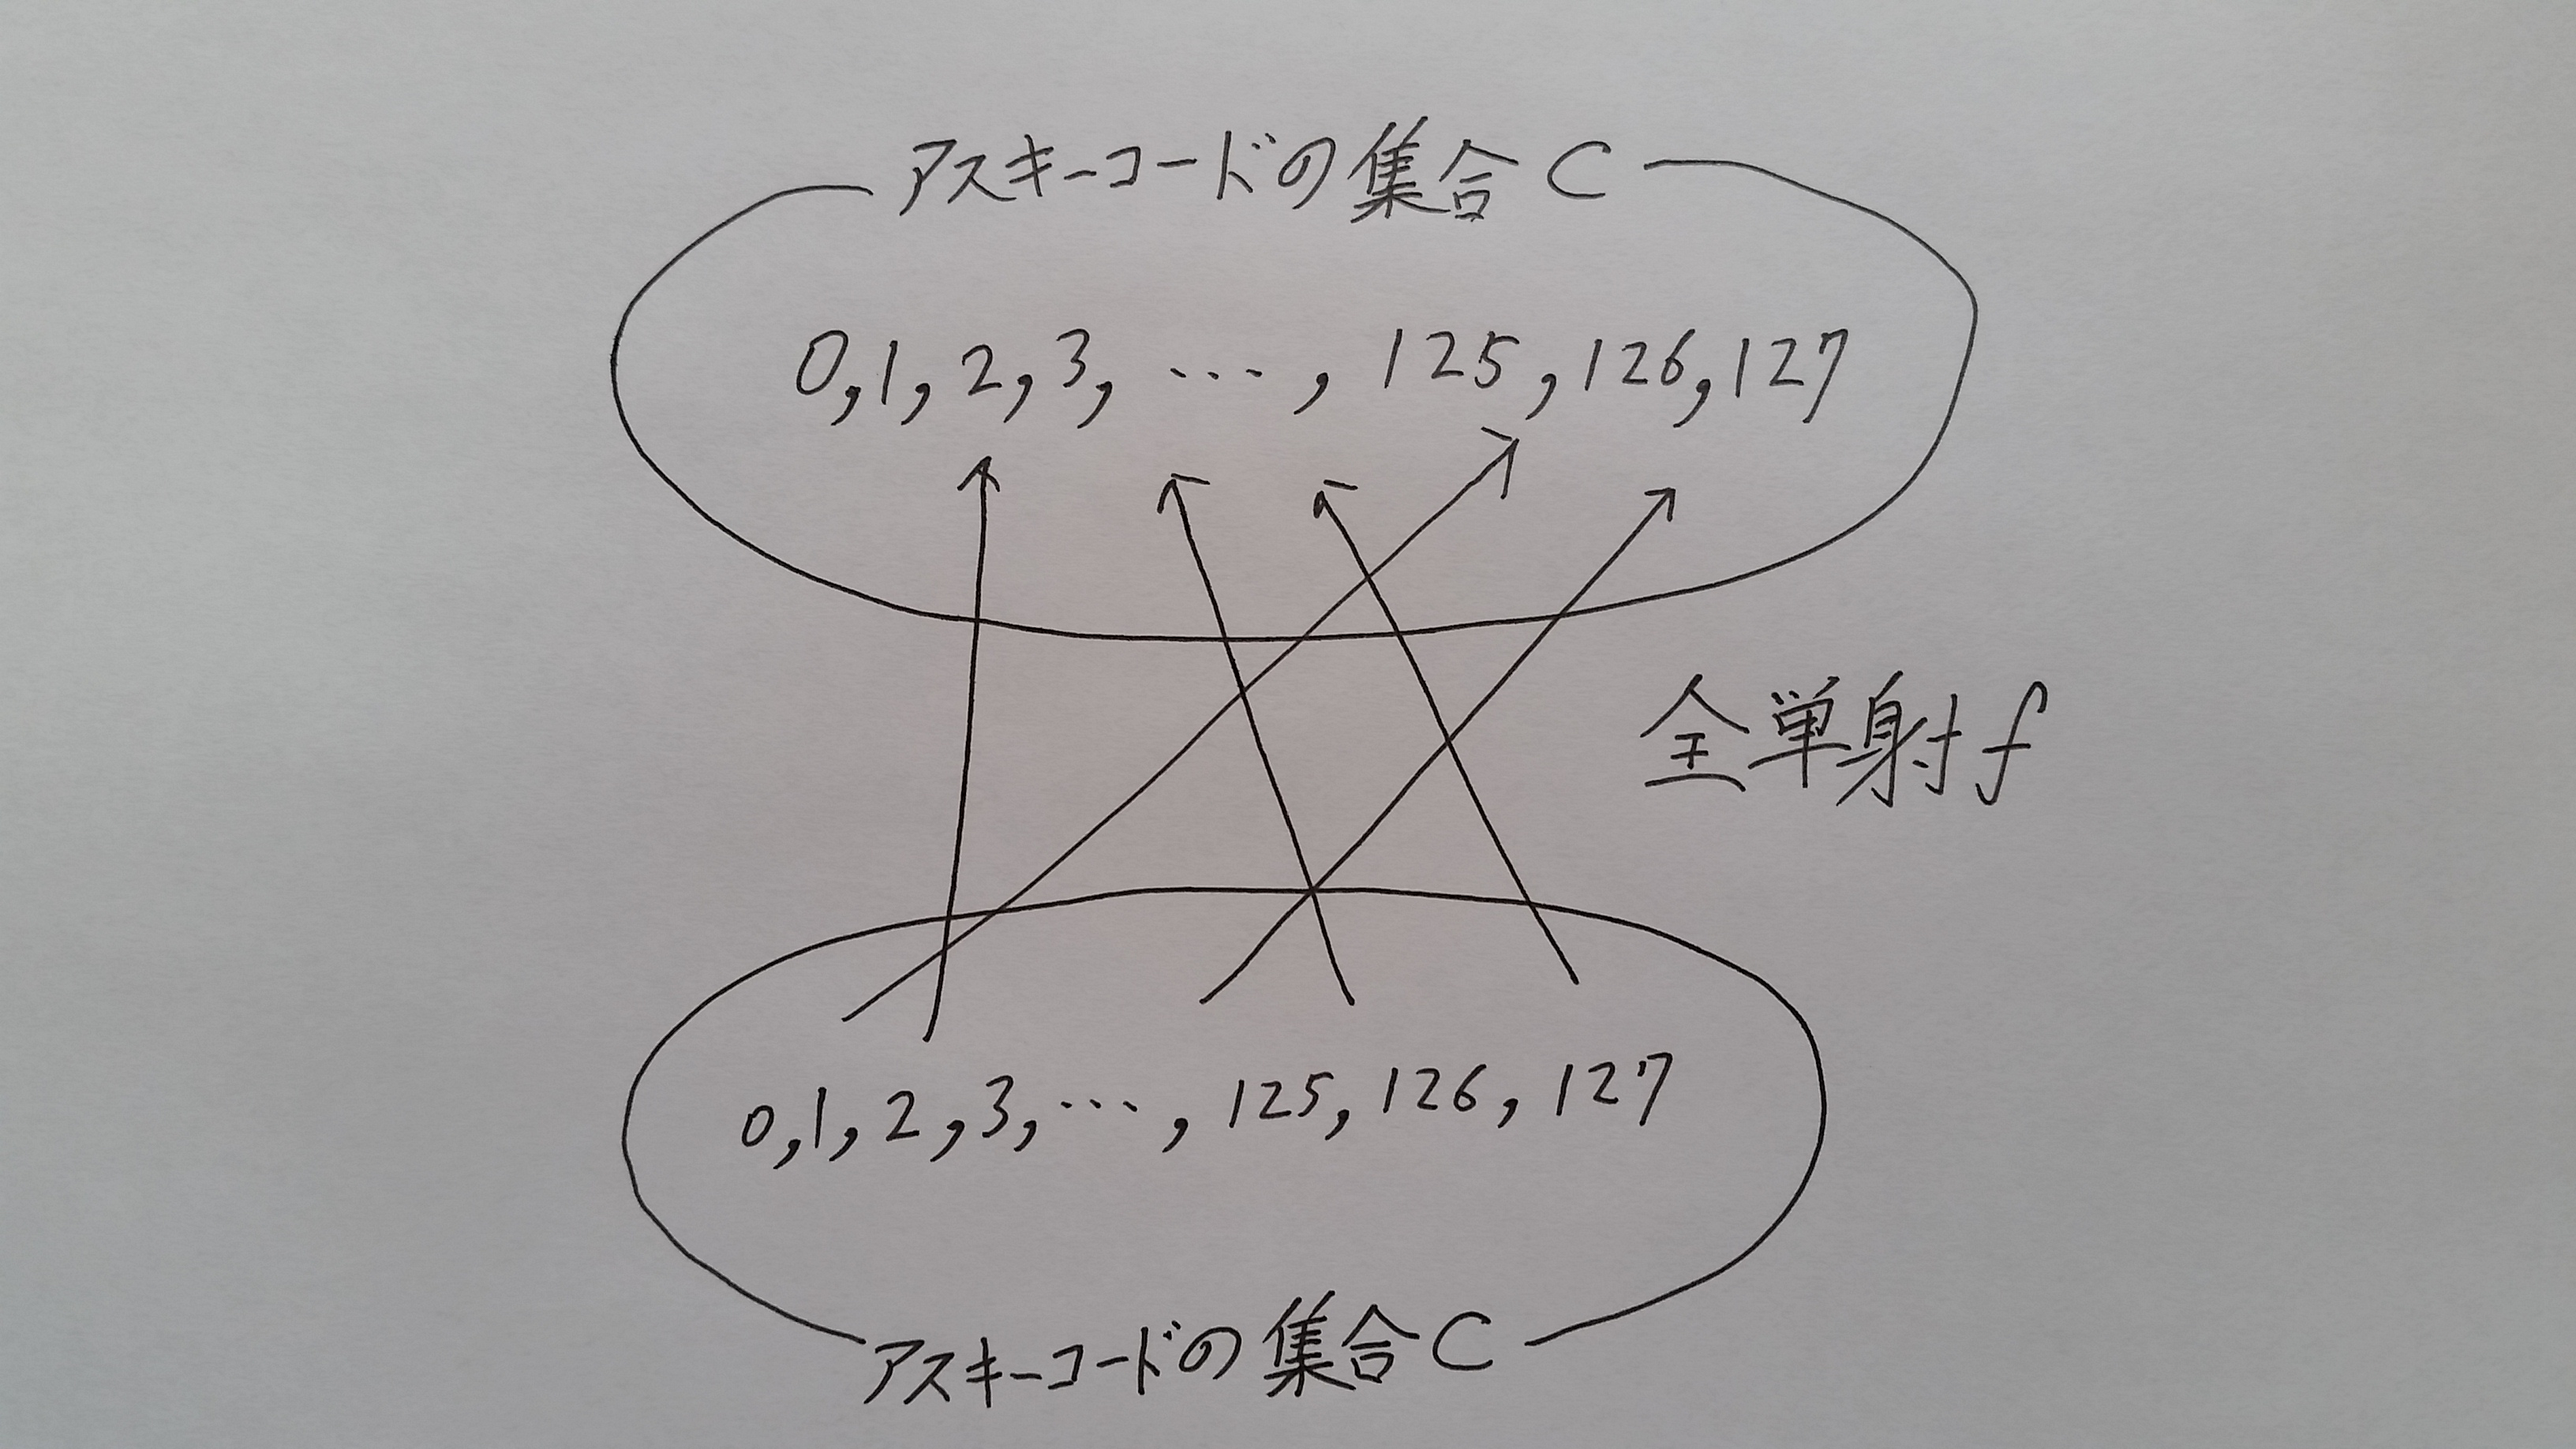
\includegraphics[width=15cm]{../caesar/algorithm.jpg}\\
このアルゴリズムに基づいて、original\_encrypt.cとoriginal\_decrypt.cを以下のように作成した。
\lstinputlisting[caption=$original\_encrypt.c$,label=OriginalEncryptC]{../caesar/original_encrypt.c}
\lstinputlisting[caption=$original\_decrypt.c$,label=OriginalDecryptC]{../caesar/original_decrypt.c}
また、共通鍵の入力が面倒なので乱数で共通鍵を作成するプログラムkey.cを以下のように作成した。
\lstinputlisting[caption=$key.c$,label=KeyC]{../caesar/key.c}
そして
\begin{lstlisting}[basicstyle=\ttfamily\footnotesize, frame=single]
gcc key.c -o key
./key > key.txt
\end{lstlisting}
を実行し、以下のようなkey.txtを得た。
\lstinputlisting[caption=$key.txt$,label=KeyTxt]{../caesar/key.txt}
そして、これを共通鍵として以下のコマンドを実行した。
\begin{lstlisting}[basicstyle=\ttfamily\footnotesize, frame=single]
gcc original_encrypt.c -o original_encrypt
gcc original_decrypt.c -o original_decrypt
./original_encrypt caesar_sample.txt original_encrypted.txt < key.txt
./original_decrypt original_encrypted.txt original_decrypted.txt < key.txt
\end{lstlisting}
original\_encrypted.txtは文字化けしているためtexで直接表示させることができなかったため、catコマンドでoriginal\_encrypted.txtを表示させた画像をここに掲載する。\\
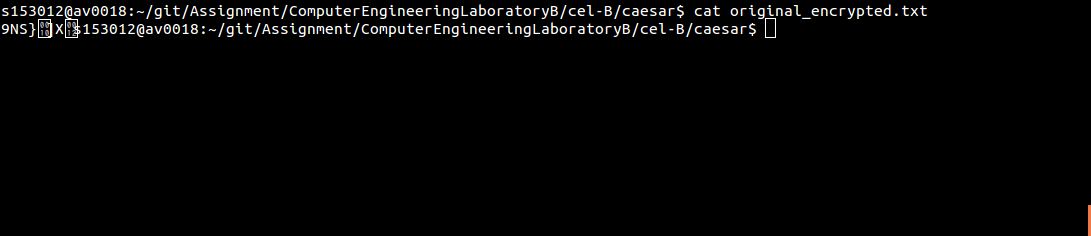
\includegraphics[width=15cm]{../caesar/original_encrypted.png}\\
original\_decrypted.txtは以下のようになっていた。\\
\lstinputlisting[caption=$original\_decrypted.txt$,label=OriginalDecryptedTxt]{../caesar/original_decrypted.txt}
%....

%%% ------------------------------------------------------------------
\newpage
\section{第4回 暗号化技術(2):公開鍵暗号}
\subsection{RSA暗号の実験(その1)}
まず、サンプルプログラムをコピーして以下のように修正した。
\lstinputlisting[caption=$rsa\_encrypt.c$,label=RSAEncryptC]{../rsa/rsa_encrypt.c}
\lstinputlisting[caption=$rsa\_decrypt.c$,label=RSADecryptC]{../rsa/rsa_decrypt.c}
これらをコンパイルしてrsa\_encryptとrsa\_decryptという実行可能ファイルを作成した。次に、以下のような原文を用意した。
\lstinputlisting[caption=$rsa\_sample.txt$,label=RSASampleTxt]{../rsa/rsa_sample.txt}
この原文に対して、$ e = 13, d = 149, n = 392 $とし、以下のコマンドで暗号化と復号化をした。
\begin{lstlisting}[basicstyle=\ttfamily\footnotesize, frame=single]
./rsa_encrypt rsa_sample.txt rsa_encrypted.txt
./rsa_decrypt rsa_encrypted.txt rsa_decrypted.txt
\end{lstlisting}
rsa\_encrypted.txtは以下のようになった。\\
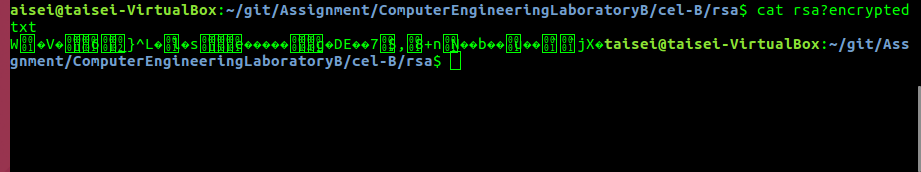
\includegraphics[width=15cm]{../rsa/rsa_encrypted.png}\\
rsa\_decrypted.txtは以下のようになった。
\lstinputlisting[caption=$rsa\_decrypted.txt$,label=RSADecryptedTxt]{../rsa/rsa_decrypted.txt}
また、鍵の効力の確認として$ d = 2, n = 202 $として以下のコマンドを実行して復号化した。
\begin{lstlisting}[basicstyle=\ttfamily\footnotesize, frame=single]
./rsa_decrypt rsa_encrypted.txt rsa_decrypted_by_wrong_keys.txt
\end{lstlisting}
rsa\_decrypted\_by\_wrong\_keys.txtは以下のようになった。\\
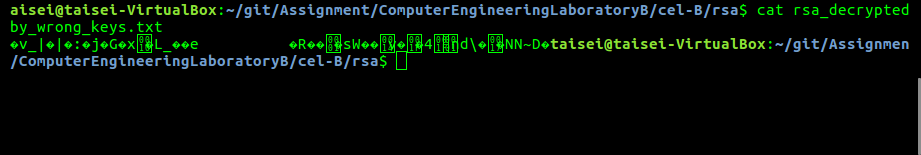
\includegraphics[width=15cm]{../rsa/rsa_decrypted_by_wrong_keys.png}\\
\subsection{RSA暗号の実験(その2)}
2つの画像clover.pngとusagi.pngをコピーして以下のコマンドを実行して、RSA暗号が画像に対しても有効であることを確認した。
\begin{lstlisting}[basicstyle=\ttfamily\footnotesize, frame=single]
./rsa_encrypt clover.png clover_encrypted.png
./rsa_encrypt usagi.png usagi_encrypted.png
./rsa_decrypt clover_encrypted.png clover_decrypted.png
./rsa_decrypt usagi_encrypted.png usagi_decrypted.png
\end{lstlisting}
clover\_encrypted.pngとusagi\_encrypted.pngは表示することが出来なかったが、clover\_decrypted.pngとusagi\_decrypted.pngはそれぞれclover.pngとusagi.pngと全く同じように表示された。 また、鍵の効力の確認として$ d = 2, n = 202 $として以下のコマンドを実行して復号化した。
\begin{lstlisting}[basicstyle=\ttfamily\footnotesize, frame=single]
./rsa_decrypt clover_encrypted.png clover_decrypted_by_wrong_keys.png
./rsa_decrypt usagi_encrypted.png usagi_decrypted_by_wrong_keys.png
\end{lstlisting}
clover\_decrypted\_by\_wrong\_keys.pngとusagi\_decrypted\_by\_wrong\_keys.pngは表示することが出来なかった。
\subsection{課題}
\begin{enumerate}
	\renewcommand{\labelenumi}{\arabic{enumi}}
	\item $ n = 15 , e = 3 , d = 3 $としたとき、6以上8以下の整数$m$について、いずれの$m$に対しても式$ c = m ^e \bmod n $及び$ m = c ^d \bmod n $が成立することを確認せよ。\\\\
$ m = 6 $のとき\\
以下のコマンドを実行して計算した。
\begin{lstlisting}[basicstyle=\ttfamily\footnotesize, frame=single]
i=6
expr $i \* $i \* $i % 15
\end{lstlisting}
結果は6だった。よって、
\begin{eqnarray}
	c & = & m ^e \bmod n \nonumber \\
	& = & 6 ^3 \bmod 15 \nonumber \\
	& = & 6 \nonumber
\end{eqnarray}
さらに、
\begin{eqnarray}
	m ^e \bmod n & = & 6 ^3 \bmod 15 \nonumber \\
	& = & 6 \nonumber \\
	& = & m \nonumber
\end{eqnarray}
よって$ m = 6 $のときに$ c = m ^e \bmod n $及び$ m = c ^d \bmod n $が成り立つことが確認できた。
$ m = 7 $のとき\\
以下のコマンドを実行して計算した。
\begin{lstlisting}[basicstyle=\ttfamily\footnotesize, frame=single]
i=7
expr $i \* $i \* $i % 15
\end{lstlisting}
結果は13だった。よって、
\begin{eqnarray}
	c & = & m ^e \bmod n \nonumber \\
	& = & 7 ^3 \bmod 15 \nonumber \\
	& = & 13 \nonumber
\end{eqnarray}
さらに、
\begin{eqnarray}
	m ^e \bmod n & = & 13 ^3 \bmod 15 \nonumber \\
	& = & 7 \nonumber \\
	& = & m \nonumber
\end{eqnarray}
よって$ m = 7 $のときに$ c = m ^e \bmod n $及び$ m = c ^d \bmod n $が成り立つことが確認できた。
$ m = 8 $のとき\\
以下のコマンドを実行して計算した。
\begin{lstlisting}[basicstyle=\ttfamily\footnotesize, frame=single]
i=8
expr $i \* $i \* $i % 15
\end{lstlisting}
結果は2だった。よって、
\begin{eqnarray}
	c & = & m ^e \bmod n \nonumber \\
	& = & 8 ^3 \bmod 15 \nonumber \\
	& = & 2 \nonumber
\end{eqnarray}
さらに、
\begin{eqnarray}
	m ^e \bmod n & = & 2 ^3 \bmod 15 \nonumber \\
	& = & 8 \nonumber \\
	& = & m \nonumber
\end{eqnarray}
よって$ m = 8 $のときに$ c = m ^e \bmod n $及び$ m = c ^d \bmod n $が成り立つことが確認できた。\\
よって$ m = 6 , m = 7 , m = 8 $のときに$ c = m ^e \bmod n $及び$ m = c ^d \bmod n $が成り立つことが確認できた。
	\item 今回の実験で用いたサンプルプログラムでは、暗号文のデータ量は原文の2倍になる。このように、RSA暗号では、正しく暗号化と復号化がなされるような公開鍵を復号鍵を作成すると、暗号文のデータ量(ビット数)は原文のデータ量(ビット数)よりも大きくなってしまう。この理由について説明せよ。\\
原文の一文字を暗号化する関数encryptの出力の最大値はRSA暗号のルールより$ n - 1 $となる。$ n $は$ m $の最大値より大きくなければならないのでRSA暗号では暗号化した時にデータ量が増える。
\end{enumerate}
% --- 参考文献リストここから
%\newpage
\begin{thebibliography}{9}
%\bibitem{book-sample} 神崎映光,西川津ビビッド,出雲島猫,「書籍の参照はこんな感じ」,島大出版,1979年.
%\bibitem{url-sample} 島根大学 総合理工学部 数理・情報システム学科(情報系),http://www.cis.shimane-u.ac.jp/.
\bibitem{suihei-parity} ネットワークの基礎知識 誤り制御について , http://www5e.biglobe.ne.jp/~komichan/network/n1\_CRC.html
\end{thebibliography}
% --- 参考文献リストここまで
%

\end{document}
